\documentclass[xcolor={x11names}]{beamer}
\usetheme{Madrid}

\usepackage{amssymb}
\usepackage{ulem}
\usepackage[utf8]{inputenc}
\usepackage{mathtools}
\usepackage{multicol}
%\usepackage[x11names]{xcolor}
\usefonttheme{professionalfonts}


% Subfigures
\usepackage{caption}
\usepackage{subcaption}




%% MATH commands
\DeclareMathOperator{\Var}{Var}


%% THEOREMS
%\newtheorem{theorem}{Theorem}
\newtheorem{thm}{Teorema}[section] % the main one
% Definición
%\theoremstyle{definition}
\newtheorem{definicion}{Definición}[section]
\newtheorem{lema}{Lema}[section]



%% PFGplots %%
\usepackage{pgfplots}

%% Exponential distribution
\pgfmathdeclarefunction{exponential}{1}{%
  \pgfmathparse{(#1)*exp(-#1*x)}%
}

%% Poisson distribution
\pgfmathdeclarefunction{poiss}{1}{%
  \pgfmathparse{(#1^x)*exp(-#1)/(x!)}%
}




\newcommand{\red}[1]{{\color{red}#1}}
\newcommand{\blue}[1]{{\color{blue}#1}}

%%%%%%%%%%
%% TIKZ %%
%%%%%%%%%%
\usepackage{tikz}
\usepackage{animate}
\usetikzlibrary{positioning}
\usetikzlibrary{shapes,arrows, positioning, calc}
\usetikzlibrary{overlay-beamer-styles}
\usetikzlibrary{chains,shapes.multipart}




%%% Insert section name before the section %%%
\AtBeginSection[]{
  \begin{frame}
  \vfill
  \centering
  \begin{beamercolorbox}[sep=8pt,center,shadow=true,rounded=true]{title}
    \usebeamerfont{title}\insertsectionhead\par%
  \end{beamercolorbox}
  \vfill
  \end{frame}
}



\title[Tema 5]{Tema 5: Introducción al {\sout{Teletráfico}}\\y a la Teoría de Colas}
\subtitle{Redes y Servicios de Telecomunicaciones (RSTC)\\
Grado en Ingeniería de Tecnologías y Servicios de Telecomunicación}
%\author{M. Saiful Bari\inst{1} \and Mr X\inst{2}}

\author{Jorge Martín Pérez\inst{1}}
\institute{
    \inst{1}
    Departamento de Ingeniería Telemática, Universidad Politécnica de Madrid
}

\date{\today}







%%%%%%%%%%%%%%%%%%%%
%%% SLIDES START %%%
%%%%%%%%%%%%%%%%%%%%
\begin{document}


%%% TITLE %%%
\frame{\titlepage}


\begin{frame}{Contenido}
    \tableofcontents
\end{frame}




\section{Introducción}
\begin{frame}{\secname}
    La teoría de colas modela:
    \begin{itemize}
        \item colas de supermercado;
        \item colas en gasolineras;
        \item colas en taquillas; o
        \item \textbf{colas de routers}.
    \end{itemize}

    \vfill
    Nos interesa saber:
    \begin{itemize}
        \item ¿cuánto vamos a esperar?; o
        \item la probabilidad de que esté llena la cola.
    \end{itemize}
\end{frame}



\begin{frame}{\secname}
    \begin{figure}
        
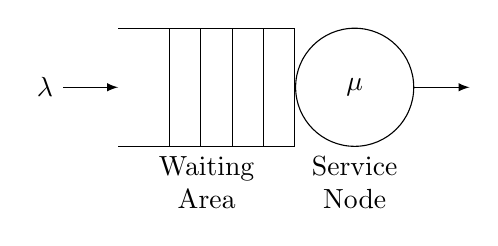
\begin{tikzpicture}[start chain=going right,>=latex,node distance=0pt]
% the rectangular shape with vertical lines
\node[rectangle split, rectangle split parts=6,
draw, rectangle split horizontal,text height=1cm,text depth=0.5cm,on chain,inner ysep=0pt] (wa) {};
\fill[white] ([xshift=-\pgflinewidth,yshift=-\pgflinewidth]wa.north west) rectangle ([xshift=-15pt,yshift=\pgflinewidth]wa.south);

% the circle
\node[draw,circle,on chain,minimum size=1.5cm] (se) {$\mu$};

% the arrows and labels
\draw[->] (se.east) -- +(20pt,0);
\draw[<-] (wa.west) -- +(-20pt,0) node[left] {$\lambda$};
\node[align=center,below] at (wa.south) {Waiting \\ Area};
\node[align=center,below] at (se.south) {Service \\ Node};
\end{tikzpicture}

    \end{figure}

    En una cola:
    \begin{itemize}
        \item llegan $\lambda$ [usuarios/sec]
        \item hay $q=4$ usuarios encolados;
        \item hay $n=5$ usuarios en total; y
        \item se sirven $\mu$ [usuarios/sec].
    \end{itemize}
\end{frame}


\begin{frame}{\secname}
    Problema:
    \begin{itemize}
        \item las llegadas; y
        \item tiempos de servicio
    \end{itemize}
    son \textbf{aleatorios}.

    \vfill

    \textit{Ejemplo}: la persona que nos
    atiende en caja tarda más o menos
    dependiendo de como de cansada esté,
    o de cuánto tarde la pasarela de pago
    (aleatorio).
\end{frame}






\section{Distribución Exponencial}

\begin{frame}{\secname}
    \begin{figure}
        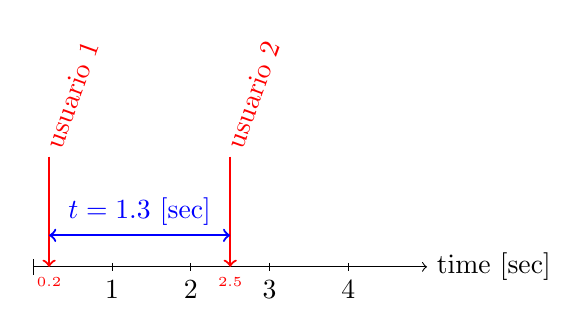
\begin{tikzpicture}
    % Time axis
    \draw[|->] (0,0) -- (5,0) node[anchor=west] {time [sec]};

    % ticks
    \draw (1,.05) -- (1,-.05) node[below] {1};
    \draw (2,.05) -- (2,-.05) node[below] {2};
    \draw (3,.05) -- (3,-.05) node[below] {3};
    \draw (4,.05) -- (4,-.05) node[below] {4};

    
    % arrivals
    \draw[->,color=red,thick] (0.2,1.4) node[anchor=west,rotate=70] {usuario 1} --(0.2,0) node[below,anchor=north] {\tiny 0.2};
    \draw[->,color=red,thick] (2.5,1.4)node[anchor=west,rotate=70] {usuario 2} --(2.5,0) node[below,anchor=north] {\tiny 2.5};

    \draw[<->,color=blue,thick] (0.2,.4) -- node[above,pos=0.5]{$t=1.3$ [sec]} (2.5,.4);
\end{tikzpicture}

    \end{figure}
    El tiempo entre los usuarios que
    llegan a la cola \blue{$t$} se puede
    modelar con la \textbf{distribución exponencial}.
\end{frame}



\begin{frame}{\secname}
    \begin{definicion}[Distribución exponencial]
        Se dice que una variable aleatoria
        continua $t\in\mathbb{N}$ sigue una
        distribución exponencial si su
        función de densidad es:
        \begin{equation}
            f_t(\tau) = \mathbb{P}(t=\tau) = \lambda e^{-\lambda \tau}
        \end{equation}
        donde $\lambda>0$ es el parámetro
        que caracteriza la distribución.
    \end{definicion}
\end{frame}




\begin{frame}{\secname: propiedades}
    \begin{figure}
        \begin{tikzpicture}

\begin{axis}[every axis plot post/.append style={
  mark=none,domain=0:3,samples=20},
  axis x line*=bottom,
  axis y line*=left,
  xlabel={$\tau$ [sec]},
  ylabel={$f_t(\tau)$},
  enlargelimits=upper,
  width=4in,
  height=2in]
  \addplot[ultra thick,smooth,color=DodgerBlue1] {exponential(1)} node [pos=0.3,anchor=south west] {$\lambda=1$};
  \addplot[ultra thick,smooth,color=DodgerBlue4] {exponential(0.5)} node [pos=0.25,anchor=north east] {$\lambda=\frac{1}{2}$};
\end{axis}


\end{tikzpicture}


    \end{figure}


    \begin{itemize}
        \item \textbf{media}: $\mathbb{E}[t]=\tfrac{1}{\lambda}$
        \item \textbf{varianza}: $\Var[t]=\tfrac{1}{\lambda^2}$
    \end{itemize}
\end{frame}




\begin{frame}{\secname: ejemplo gasolinera}
    \textit{Ejemplo}: el tiempo medio
    que pasa un coche en un surtidor es
    $\mathbb{E}[\blue{t}]=\tfrac{1}{\lambda}=2$ [min].
    Por tanto $\lambda=\tfrac{1}{2}$ [coches/min].

    \vfill


    \begin{figure}
     \centering
     \begin{subfigure}[b]{0.45\textwidth}
         \centering
         \resizebox{\textwidth}{!}{%
             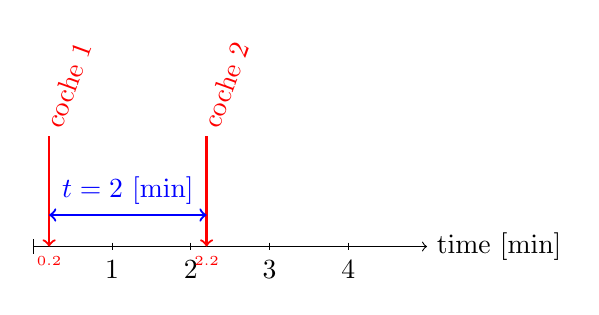
\begin{tikzpicture}
    % Time axis
    \draw[|->] (0,0) -- (5,0) node[anchor=west] {time [min]};

    % ticks
    \draw (1,.05) -- (1,-.05) node[below] {1};
    \draw (2,.05) -- (2,-.05) node[below] {2};
    \draw (3,.05) -- (3,-.05) node[below] {3};
    \draw (4,.05) -- (4,-.05) node[below] {4};

    
    % arrivals
    \draw[->,color=red,thick] (0.2,1.4) node[anchor=west,rotate=70] {coche 1} --(0.2,0) node[below,anchor=north] {\tiny 0.2};
    \draw[->,color=red,thick] (2.2,1.4)node[anchor=west,rotate=70] {coche 2} --(2.2,0) node[below,anchor=north] {\tiny 2.2};

    \draw[<->,color=blue,thick] (0.2,.4) -- node[above,pos=0.5]{$t=2$ [min]} (2.2,.4);
\end{tikzpicture}
%
         }
         \caption{$\mathbb{P}(\blue{t=2})=\tfrac{1}{2}\ e^{\frac{1}{2}\cdot \blue{2}}=0.18$}
     \end{subfigure}
     \hfill
     \begin{subfigure}[b]{0.45\textwidth}
         \centering
         \resizebox{\textwidth}{!}{%
             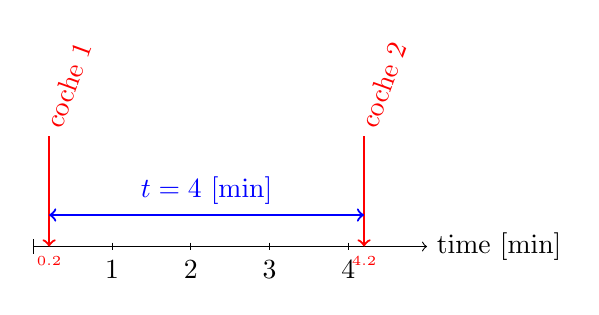
\begin{tikzpicture}
    % Time axis
    \draw[|->] (0,0) -- (5,0) node[anchor=west] {time [min]};

    % ticks
    \draw (1,.05) -- (1,-.05) node[below] {1};
    \draw (2,.05) -- (2,-.05) node[below] {2};
    \draw (3,.05) -- (3,-.05) node[below] {3};
    \draw (4,.05) -- (4,-.05) node[below] {4};

    
    % arrivals
    \draw[->,color=red,thick] (0.2,1.4) node[anchor=west,rotate=70] {coche 1} --(0.2,0) node[below,anchor=north] {\tiny 0.2};
    \draw[->,color=red,thick] (4.2,1.4)node[anchor=west,rotate=70] {coche 2} --(4.2,0) node[below,anchor=north] {\tiny 4.2};

    \draw[<->,color=blue,thick] (0.2,.4) -- node[above,pos=0.5,anchor=south]{$t=4$ [min]} (4.2,.4);
\end{tikzpicture}
%
         }
         \caption{$\mathbb{P}(\blue{t=4})=\tfrac{1}{2}\ e^{-\frac{1}{2}\cdot \blue{4}}=0.07$}
     \end{subfigure}
    \end{figure}

\end{frame}





\subsection{Propiedad sin memoria}


\begin{frame}{\secname: \subsecname}
Si ya han pasado {\color{DodgerBlue1}$s$ [sec]}, ¿cuál es
    la probabilidad de que tarde {\color{DodgerBlue4}$\tau$
    [sec]} más?:
    \begin{equation}
        \mathbb{P}(\red{t}>{\color{DodgerBlue1}s}+{\color{DodgerBlue4}\tau}|\ \red{t}>{\color{DodgerBlue1}s})
    \end{equation}

    \vfill

    \begin{figure}
        \begin{tikzpicture}

    % Already passed
    \draw[draw=none,fill=DodgerBlue1!20] (0.2,0) rectangle ++(1,1.4);

    % Time axis
    \draw[|->] (0,0) -- (5,0) node[anchor=west] {time [sec]};

    % ticks
    \draw (1,.05) -- (1,-.05) node[below] {1};
    \draw (2,.05) -- (2,-.05) node[below] {2};
    \draw (3,.05) -- (3,-.05) node[below] {3};
    \draw (4,.05) -- (4,-.05) node[below] {4};
    
    % arrivals
    \draw[->,color=red,thick] (0.2,2) node[anchor=west,rotate=70] {coche 1} --(0.2,0) node[below,anchor=north] {\tiny 0.2};
    \draw[-,color=DodgerBlue1,dashed] (1.2,1.4) --(1.2,0) node[below,anchor=north] {\tiny 1.2};
    \draw[-,color=DodgerBlue4,dashed] (4.2,1.4) --(4.2,0) node[below,anchor=north] {\tiny 4.2};

    \draw[->,color=red,thick,visible on=<2>] (4.5,2.2)node[anchor=west,rotate=70] {coche 2} --(4.5,0.2) ;

    \draw[<->,color=DodgerBlue1,thick] (0.2,.4) -- node[above,pos=0.48,anchor=south]{$s=1$} (1.2,.4);
    \draw[<->,color=DodgerBlue4,thick] (1.2,.4) -- node[above,pos=0.5,anchor=south]{$\tau=3$ [sec]} (4.2,.4);
    \draw[<->,color=red,thick, visible on=<2>] (0.2,1.7) -- node[above,pos=0.5,anchor=south]{$t$} (4.5,1.7);
\end{tikzpicture}

    \end{figure}
\end{frame}



\begin{frame}{\secname: \subsecname}
    Por la propiedad sin memoria de una
    exponencial tenemos que:
    \begin{equation}
        \mathbb{P}(\red{t}>{\color{DodgerBlue1}s}+{\color{DodgerBlue4}\tau}|\ \red{t}>{\color{DodgerBlue1}s}) = \mathbb{P}(\red{t}>{\color{DodgerBlue4}\tau})
    \end{equation}

    \vfill


    \begin{figure}
     \centering
     \begin{subfigure}[b]{0.45\textwidth}
         \centering
         \resizebox{\textwidth}{!}{%
             \begin{tikzpicture}

    % Already passed
    \draw[draw=none,fill=DodgerBlue1!20] (0.2,0) rectangle ++(1,1.4);

    % Time axis
    \draw[|->] (0,0) -- (5,0) node[anchor=west] {time [sec]};

    % ticks
    \draw (1,.05) -- (1,-.05) node[below] {1};
    \draw (2,.05) -- (2,-.05) node[below] {2};
    \draw (3,.05) -- (3,-.05) node[below] {3};
    \draw (4,.05) -- (4,-.05) node[below] {4};
    
    % arrivals
    \draw[->,color=red,thick] (0.2,2) node[anchor=west,rotate=70] {coche 1} --(0.2,0) node[below,anchor=north] {\tiny 0.2};
    \draw[-,color=DodgerBlue1,dashed] (1.2,1.4) --(1.2,0) node[below,anchor=north] {\tiny 1.2};
    \draw[-,color=DodgerBlue4,dashed] (4.2,1.4) --(4.2,0) node[below,anchor=north] {\tiny 4.2};

    \draw[->,color=red,thick] (4.5,2.2)node[anchor=west,rotate=70] {coche 2} --(4.5,0.2) ;

    \draw[<->,color=DodgerBlue1,thick] (0.2,.4) -- node[above,pos=0.48,anchor=south]{$s=1$} (1.2,.4);
    \draw[<->,color=DodgerBlue4,thick] (1.2,.4) -- node[above,pos=0.5,anchor=south]{$\tau=3$ [sec]} (4.2,.4);
    \draw[<->,color=red,thick] (0.2,1.7) -- node[above,pos=0.5,anchor=south]{$t$} (4.5,1.7);
\end{tikzpicture}
%
         }
         \caption{$\mathbb{P}(\red{t}>{\color{DodgerBlue1}s}+{\color{DodgerBlue4}\tau}|\ \red{t}>{\color{DodgerBlue1}s})$}
     \end{subfigure}
     \hfill
     \begin{subfigure}[b]{0.45\textwidth}
         \centering
         \resizebox{\textwidth}{!}{%
             \begin{tikzpicture}

    % Time axis
    \draw[|->] (0,0) -- (5,0) node[anchor=west] {time [sec]};

    % ticks
    \draw (1,.05) -- (1,-.05) node[below] {1};
    \draw (2,.05) -- (2,-.05) node[below] {2};
    \draw (3,.05) -- (3,-.05) node[below] {3};
    \draw (4,.05) -- (4,-.05) node[below] {4};
    
    % arrivals
    \draw[->,color=red,thick] (0.2,2) node[anchor=west,rotate=70] {coche 1} --(0.2,0) node[below,anchor=north] {\tiny 0.2};
    \draw[-,color=DodgerBlue4,dashed] (3.2,1.4) --(3.2,0) node[below,anchor=north] {\tiny 3.2};

    \draw[->,color=red,thick] (3.7,2.2)node[anchor=west,rotate=70] {coche 2} --(3.7,0.2) ;

    \draw[<->,color=DodgerBlue4,thick] (0.2,.4) -- node[above,pos=0.5,anchor=south]{$\tau=3$ [sec]} (3.2,.4);
    \draw[<->,color=red,thick] (0.2,1.7) -- node[above,pos=0.5,anchor=south]{$t$} (3.7,1.7);
\end{tikzpicture}
%
         }
         \caption{$\mathbb{P}(\red{t}>{\color{DodgerBlue4}\tau})$}
     \end{subfigure}
    \end{figure}
\end{frame}


\begin{frame}{\secname: \subsecname}
    \textit{Ejemplo}: en media el surtidor
    de una gasolinera está ocupado 5 [min].
    Si el surtidor lleva
    {\color{DodgerBlue1}$s=1$ [min]} ocupado,
    ¿cuál es la probabildad de que esté ocupado
    {\color{DodgerBlue4}$\tau=3$ [min]} más?

    \vfill

    Por la propiedad sin memoria tenemos:
    \begin{equation*}
        \mathbb{P}(\red{t}>{\color{DodgerBlue1}s}+{\color{DodgerBlue4}\tau}|\ \red{t}>{\color{DodgerBlue1}s}) = \mathbb{P}(\red{t}>{\color{DodgerBlue4}\tau}) = \mathbb{P}(\red{t}>{\color{DodgerBlue4}3}) = \frac{1}{5}e^{-\frac{1}{5}\cdot3} = 0.11
    \end{equation*}

\end{frame}




\subsection{Mínimo de variables exponenciales}

\begin{frame}{\secname: \subsecname}
    \textit{Ejemplo}: los compactos llegan
    a gasolinera con tasa
    {\color{Firebrick1}$\lambda_1=\tfrac{1}{4}$
    [coches/min]}, y los todoterreno con tasa
    {\color{Firebrick4}$\lambda_2=\tfrac{1}{8}$ [coches/min]}.

    \vfill

    ¿Con qué probabilidad llegua
    un coche cualquiera en 3 [min]?
\end{frame}



\begin{frame}{\secname: \subsecname}
    \begin{lema}[Mínimo de v.a. exponenciales]
        Sean las v.a.\footnote{v.a. significa variable aleatoria} exponenciales
        {\color{Firebrick1}$t_1$} y
        {\color{Firebrick4}$t_2$}, con
        tasas
        {\color{Firebrick1}$\lambda_1$} y
        {\color{Firebrick4}$\lambda_2$}; la v.a.
        $t=\min\{{\color{Firebrick1}t_1},{\color{Firebrick4}t_2}\}$
        se distribuye como una v.a. exponencial
        de tasa
        {$\lambda=\color{Firebrick1}\lambda_1+ \color{Firebrick4}\lambda_2$}.
    \end{lema}

    \vfill

    \textit{Demostración}:
    \begin{multline*}
        \mathbb{P}(t>\tau) =
        \mathbb{P}({\color{Firebrick1}t_1}>\tau)\mathbb{P}({\color{Firebrick4}t_2}>\tau)
        = \left(\int_\tau^\infty {\color{Firebrick1}\lambda_1}e^{-{\color{Firebrick1}\lambda_1} t}\ dt \right)
        \left(\int_\tau^\infty {\color{Firebrick4}\lambda_2}e^{-{\color{Firebrick4}\lambda_2} t}\ dt \right)\\
        = e^{-{\color{Firebrick1}\lambda_1} \tau} e^{-{\color{Firebrick4}\lambda_2} \tau} = e^{-({\color{Firebrick1}\lambda_1}+{\color{Firebrick4}\lambda_2})\tau}
        = e^{-\lambda \tau}
    \end{multline*}
\end{frame}




\begin{frame}{\secname: \subsecname}
    \textit{Ejemplo}: los compactos llegan
    a gasolinera con tasa
    {\color{Firebrick1}$\lambda_1=\tfrac{1}{4}$
    [coches/min]}, y los todoterreno con tasa
    {\color{Firebrick4}$\lambda_2=\tfrac{1}{8}$ [coches/min]}.

    \vfill

    ¿Con qué probabilidad llega
    un coche cualquiera en 3 [min]?

    \begin{align*}
        1-\mathbb{P}(t>1)&=1-
        ({\color{Firebrick1}\lambda_1}+
        {\color{Firebrick4}\lambda_2})
        e^{-({\color{Firebrick1}\lambda_1}+
        {\color{Firebrick4}\lambda_2})\cdot 3}\\
        & =
        1 - \left({\color{Firebrick1}\frac{1}{4}}+
        {\color{Firebrick4}\frac{1}{8}}\right)
        e^{-({\color{Firebrick1}\frac{1}{4}}+
        {\color{Firebrick4}\frac{1}{8}})\cdot 3}
        = 0.12
    \end{align*}
\end{frame}







\subsection{Comparación de exponenciales}


\begin{frame}{\secname: \subsecname}
    \textit{Ejemplo}: los compactos llegan
    a gasolinera con tasa
    {\color{Firebrick1}$\lambda_1=\tfrac{1}{4}$
    [coches/min]}, y los todoterreno con tasa
    {\color{Firebrick4}$\lambda_2=\tfrac{1}{8}$ [coches/min]}.

    \vfill

    ¿Cuál es la probabilidad de que llegue
    antes un compacto, es decir,
    (${\color{Firebrick1}t_1}<
    {\color{Firebrick4}t_2}$)?

    \begin{figure}
        \begin{tikzpicture}
    % Time axis
    \draw[|->] (0,0) -- (5,0) node[anchor=west] {time [min]};

    % ticks
    \draw (1,.05) -- (1,-.05);
    \draw (2,.05) -- (2,-.05);
    \draw (3,.05) -- (3,-.05);

    
    % arrivals
    \draw[->,color=Firebrick1,thick] (1.2,1) node[anchor=west,rotate=30] {compacto} --(1.2,0);
    \draw[->,color=Firebrick4,thick] (2,1) node[anchor=west,rotate=30] {todoterreno} --(2,0);

    % times
    \draw[<->,color=Firebrick1,thick] (0,0.35) -- node[above] {$t_1$} (1.2,0.35);
    \draw[<->,color=Firebrick4,thick] (0,-0.35) -- node[below] {$t_1$} (2,-0.35);

\end{tikzpicture}

    \end{figure}

\end{frame}



\begin{frame}{\secname: \subsecname}
    \begin{lema}[Comparación de v.a. exponenciales]
        Sean las v.a. exponenciales
        {\color{Firebrick1}$t_1$} y
        {\color{Firebrick4}$t_2$}, con
        tasas
        {\color{Firebrick1}$\lambda_1$} y
        {\color{Firebrick4}$\lambda_2$}; se
        tiene que:
        \begin{equation}
            \mathbb{P}({\color{Firebrick1}t_1}<{\color{Firebrick4}t_2}) = \frac{{\color{Firebrick1}\lambda_1}}{{\color{Firebrick1}\lambda_1}+{\color{Firebrick4}\lambda_2}}
        \end{equation}
    \end{lema}

    \vfill

    \textit{Demostración}:
    \begin{equation*}
        \mathbb{P}({\color{Firebrick1}t_1}<{\color{Firebrick4}t_2})=
        \int_0^\infty \mathbb{P}({\color{Firebrick1}t_1}=t)\mathbb{P}({\color{Firebrick4}t_2}>t)\ dt = \int_0^\infty {\color{Firebrick1}\lambda_1} e^{-{\color{Firebrick1}\lambda_1} t} e^{-{\color{Firebrick4}\lambda_2} t}\ dt = \frac{{\color{Firebrick1}\lambda_1}}{{\color{Firebrick1}\lambda_1}+{\color{Firebrick4}\lambda_2}}
    \end{equation*}
\end{frame}





\begin{frame}{\secname: \subsecname}
    \textit{Ejemplo}: los compactos llegan
    a gasolinera con tasa
    {\color{Firebrick1}$\lambda_1=\tfrac{1}{4}$
    [coches/min]}, y los todoterreno con tasa
    {\color{Firebrick4}$\lambda_2=\tfrac{1}{8}$ [coches/min]}.

    \vfill

    ¿Cuál es la probabilidad de que llegue
    antes un compacto, es decir,
    (${\color{Firebrick1}t_1}<
    {\color{Firebrick4}t_2}$)?

    \begin{figure}
        \begin{tikzpicture}
    % Time axis
    \draw[|->] (0,0) -- (5,0) node[anchor=west] {time [min]};

    % ticks
    \draw (1,.05) -- (1,-.05);
    \draw (2,.05) -- (2,-.05);
    \draw (3,.05) -- (3,-.05);

    
    % arrivals
    \draw[->,color=Firebrick1,thick] (1.2,1) node[anchor=west,rotate=30] {compacto} --(1.2,0);
    \draw[->,color=Firebrick4,thick] (2,1) node[anchor=west,rotate=30] {todoterreno} --(2,0);

    % times
    \draw[<->,color=Firebrick1,thick] (0,0.35) -- node[above] {$t_1$} (1.2,0.35);
    \draw[<->,color=Firebrick4,thick] (0,-0.35) -- node[below] {$t_1$} (2,-0.35);

\end{tikzpicture}

    \end{figure}

    \begin{equation}
        \mathbb{P}({\color{Firebrick1}t_1}<{\color{Firebrick4}t_2}) = \frac{{\color{Firebrick1}\lambda_1}}{{\color{Firebrick1}\lambda_1}+{\color{Firebrick4}\lambda_2}} = 
        \frac{{\color{Firebrick1}\frac{1}{4}}}{{\color{Firebrick1}\frac{1}{4}}+{\color{Firebrick4}\frac{1}{8}}} = 0.67
    \end{equation}

\end{frame}







\section{Procesos de llegada de Poisson}



\begin{frame}{\secname}
    \begin{figure}
        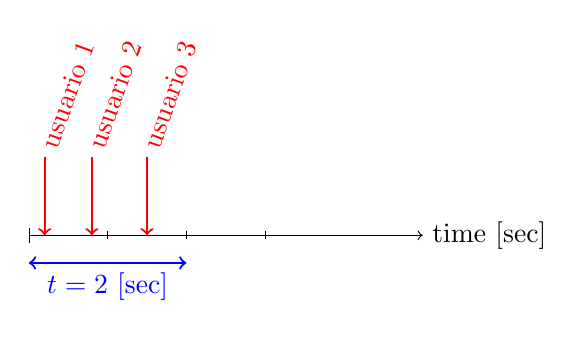
\begin{tikzpicture}
    % Time axis
    \draw[|->] (0,0) -- (5,0) node[anchor=west] {time [sec]};

    % ticks
    \draw (1,.05) -- (1,-.05);
    \draw (2,.05) -- (2,-.05);
    \draw (3,.05) -- (3,-.05);

    
    % arrivals
    \draw[->,color=red,thick] (0.2,1) node[anchor=west,rotate=70] {usuario 1} --(0.2,0);
    \draw[->,color=red,thick] (0.8,1) node[anchor=west,rotate=70] {usuario 2} --(0.8,0);
    \draw[->,color=red,thick] (1.5,1)node[anchor=west,rotate=70] {usuario 3} --(1.5,0);

    \draw[<->,color=blue,thick] (0,-.35) -- node[anchor=north,pos=0.5]{$t=2$ [sec]} (2,-.35);
\end{tikzpicture}

    \end{figure}

    Queremos saber la probabilidad de que
    lleguen 3 usuarios en 2 segundos.

    Esa probabilidad nos la da la distribución
    de Poisson si:
    \begin{itemize}
        \item llegadas \textbf{equiprobables}; y
        \item llegadas \textbf{independientes}.
    \end{itemize}
\end{frame}


\begin{frame}{\secname}
    Un proceso de llegadas de Poisson nos
    dice la probabilidad de que lleguen
    $k$ usuarios en $t$ segundos:
    \begin{equation}
        \mathbb{P}(\red{k}\ \text{usuarios en}\ \blue{t})=\frac{(\lambda \blue{t})^\red{k} e^{-\lambda \blue{t} }}{\red{k}!}
        \label{eq:poisson}
    \end{equation}
    donde $\lambda$ es la \textbf{tasa}
    de llegadas [usuarios/sec].

    \vfill

    \textit{Ejemplo}: si la tasa
    de llegada es $\lambda=5$ [usuarios/sec],
    la probabilidad de
    que lleguen $\red{k=3}$ usuarios en $\blue{t=2}$~sec es
    $\tfrac{(5\cdot2)^3 e^{-5\cdot2}}{3!}=0.0075$.
\end{frame}




\begin{frame}{\secname}
    Propiedades de la distribución de Poisson:
    \begin{itemize}
        \item \textbf{media}: $\mathbb{E}[\text{\#usuarios en}\ t\ \text{sec}]=\lambda t$ usuarios
        \item \textbf{varianza}: $\Var[\text{\#usuarios en}\ t\ \text{sec}]=\lambda t$ usuarios\textsuperscript{2}
    \end{itemize}

    \begin{figure}
        \begin{tikzpicture}

\begin{axis}[every axis plot post/.append style={
  mark=none,domain=0:20,samples=20},
  axis x line*=bottom,
  axis y line*=left,
  xlabel={$k$ [usuarios]},
  ylabel={$\mathbb{P}(k\ \text{usuarios en 1 sec})$},
  enlargelimits=upper,
  width=4in,
  height=2in]
  \addplot[ultra thick,smooth,color=HotPink2] {poiss(1)} node [pos=0.03,anchor=south west] {$\lambda=1$};
  \addplot[ultra thick,smooth,color=HotPink3] {poiss(5)} node [pos=0.24,anchor=south west] {$\lambda=5$};
  \addplot[ultra thick,smooth,color=HotPink4] {poiss(10)} node [pos=0.65,anchor=south west] {$\lambda=10$};
\end{axis}


\end{tikzpicture}


    \end{figure}
\end{frame}


\begin{frame}{\secname}
    ¿Cómo se distribuyen las llegadas
    de \textbf{\color{Firebrick1}A} y
    \textbf{\color{Firebrick4}B} juntos?

    \begin{figure}
        \begin{tikzpicture}
    % Time axis
    \draw[|->] (0,0) -- (5,0) node[anchor=west] {time [sec]};

    % ticks
    \draw (1,.05) -- (1,-.05) node[pos=1,anchor=north] {1};
    \draw (2,.05) -- (2,-.05) node[pos=1,anchor=north] {2};
    \draw (3,.05) -- (3,-.05) node[pos=1,anchor=north] {3};
    \draw (4,.05) -- (4,-.05) node[pos=1,anchor=north] {4};

    
    % arrivals A
    \draw[->,color=Firebrick1,thick] (0.2,1) node[anchor=west,rotate=70] {usuario A.1} --(0.2,0);
    \draw[->,color=Firebrick4,thick] (0.8,1) node[anchor=west,rotate=70] {usuario B.1} --(0.8,0);
    \draw[->,color=red,thick] (1.5,1)node[anchor=west,rotate=70] {usuario A.2} --(1.5,0);
    \draw[->,color=red,thick] (3,1)node[anchor=west,rotate=70] {usuario A.3} --(3,0);
    \draw[->,color=Firebrick4,thick] (3.8,1) node[anchor=west,rotate=70] {usuario B.2} --(3.8,0);

\end{tikzpicture}

    \end{figure}

    Vemos que:
    \begin{itemize}
        \item {\color{Firebrick1}$\lambda_A=\tfrac{3}{4}$} [usuarios/sec], ya que {\color{Firebrick1}$N_A(t=4sec)=3$} [usuarios]
        \item {\color{Firebrick4}$\lambda_B=\tfrac{2}{4}$} [usuarios/sec], ya que {\color{Firebrick4}$N_B(t=4sec)=2$} [usuarios]
    \end{itemize}

\end{frame}



\begin{frame}{\secname}
    \begin{thm}[Palm-Khintchine{\color{red}Put Pablos' ref}]
        Sea $\{N_i(t)\}_i$ un conjunto de $n$
        procesos de llegada independientes
        con sendas tasas
        $\lambda_i$.
        La superposición de procesos
        \begin{equation}
            N(t)=\sum_i^n N_i(t), t\geq0
        \end{equation}
        tiende a un \textbf{proceso de Poisson}
        de tasa $\lambda=\sum_i \lambda_i$
        cuando $n\to\infty$, siempre y cuando
        se cumpla:
        \begin{enumerate}
            \item carga finita $\lambda<\infty$; y
            \item ningún proceso domine al
                agregado $\lambda_i<<\lambda$
        \end{enumerate}
    \end{thm}
    
\end{frame}



\section{Sistema M/M/1}



\end{document}
